\subsection{Beskrivelse}

\paragraph{Brukergrensesnitt}
Brukergrensesnittet for å se status på bilen og løpet er ikke noe nytt system. 
Det ble laget et system av en tidligere EiT gruppe, dette systemet er laget ved hjelp av java og viser følgende data:
\begin{itemize}
\item Kart med bil
\item Hastighet
\item Grafer med måledata
\item Noen reléer
\end{itemize}
Et skjermbilde av dette er gjengitt i \ref{fig:gammeljava}.

\begin{figure}[H]
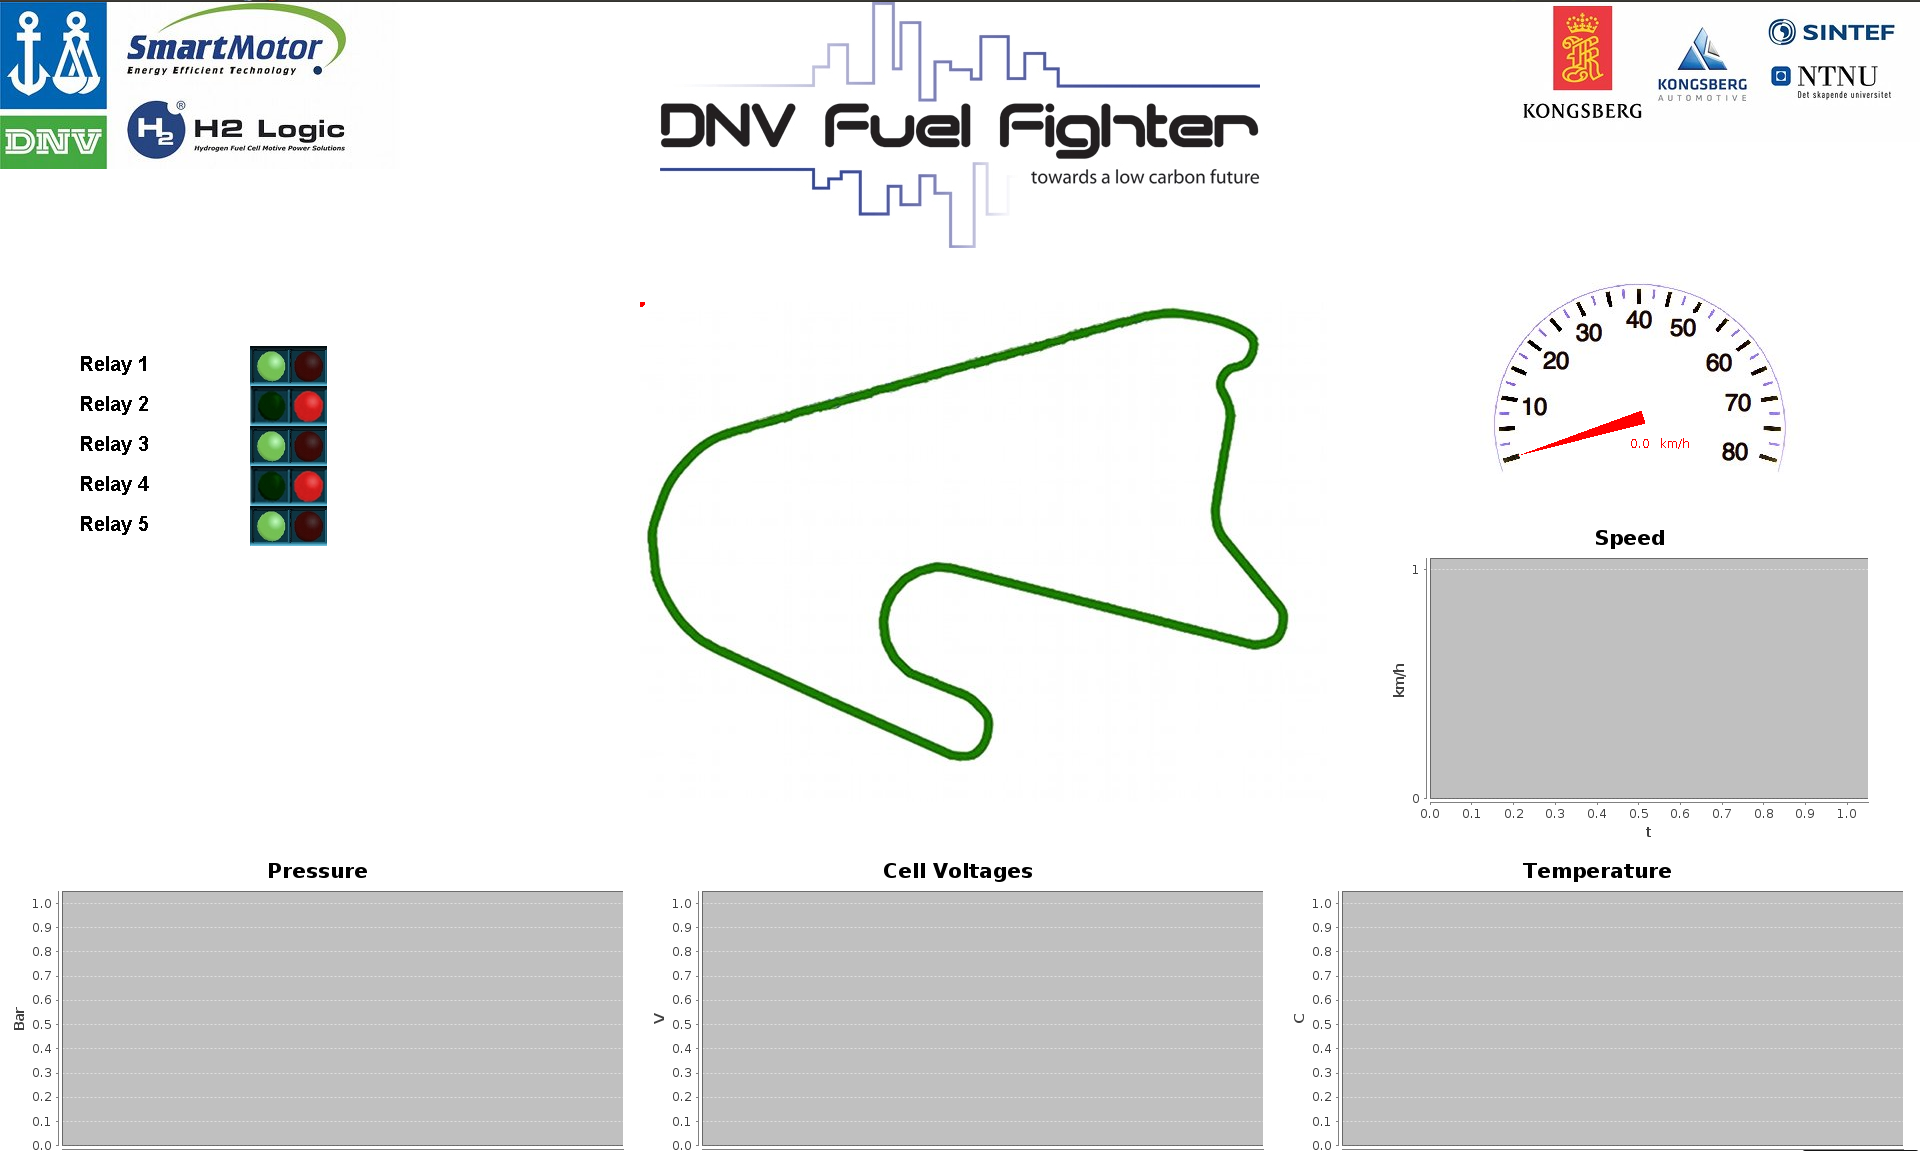
\includegraphics[width=\textwidth]{images/java.png}
\caption{Eksisterende system}
\label{fig:gammeljava}
\end{figure}

\paragraph{Telemetrimodul}
Modulen som sitter i bilen og sender data ble laget av Anders Guldahl i 2009 \cite{telemetrithesis}, denne leser forskjellige parametre fra resten av bilen og sender dette over GPRS til en server.

\subsection{Problemer og ulemper}
\paragraph{Brukergrensesnitt}
Det ble funnet noen problemer ved det eksisterende systemet:
\begin{itemize}
\item Har ikke mulighet til å vise kart for hvor bilen er annet enn på banen.
\item Kan ikke vise historie på måledata.
\item Kun for bruk internt med Ecomarathon, kan ikke brukes f.eks. i PR sammenheng på nett.
\item Fungerte ikke under selve løpet. Det mistenkes at dette skyldtes bilen og ikke systemet, men ingen vet sikkert.
\item Ingen på prosjektet vet hvordan det brukes
\end{itemize}
I tillegg til dette kom det ønsker om hvordan det skal se ut fra resten av Ecomarathon teamet som er vanskelig å oppfylle i det eksisterende systemet.

\paragraph{Telemetrimodul}
Telemetrimodulen har noen svakheter som må løses før den fungerer slik den skal.
Ved konkurransen i fjor sendte ikke bilen data når den var i Tyskland.
Telemtrimodulen har heller ikke implementert at den skal sende data om posisjon og hastighet.